\documentclass[journal,onecolumn,12pt]{IEEEtran}
\IEEEoverridecommandlockouts
% The preceding line is only needed to identify funding in the first footnote. If that is unneeded, please comment it out.
\usepackage{cite}
\usepackage[numbers]{natbib}
\usepackage{amsmath,amssymb,amsfonts}
%\usepackage{algorithmic}
\usepackage{graphicx}
\usepackage{subcaption}
\usepackage{textcomp}
\usepackage{xcolor}
\def\BibTeX{{\rm B\kern-.05em{\sc i\kern-.025em b}\kern-.08em
    T\kern-.1667em\lower.7ex\hbox{E}\kern-.125emX}}

\usepackage[acronym]{glossaries}
% abbreviations:
\newacronym{cnn}{CNN}{Convolution Neural Network}
\newacronym{yolov3}{YOLOv3}{You Look Only Once v3}
\newacronym{hog}{HOG}{Histogram of Oriented Gradients}
\newacronym{surf}{SURF}{Speeded-Up Robust Features}
\newacronym{lbp}{LBP}{Local Binary Patterns}
\begin{document}

\title{The nut job\\
{\footnotesize }%\textsuperscript{*}Note: Sub-titles are not captured in Xplore and should not be used}
\thanks{Identify applicable funding agency here. If none, delete this.}
}

\author{\IEEEauthorblockN{1\textsuperscript{st} Priteshkumar Gohil}
\IEEEauthorblockA{\textit{Department of Computer Science} \\
\textit{Hochschule Bonn-Rhein-Sieg}\\
Bonn, Germany\\
priteshbgohil@gmail.com}
%\and
%\IEEEauthorblockN{2\textsuperscript{nd} Given Name Surname}
%\IEEEauthorblockA{\textit{dept. name of organization (of Aff.)} \\
%\textit{name of organization (of Aff.)}\\
%City, Country \\
%email address}
%\and
%\IEEEauthorblockN{3\textsuperscript{rd} Given Name Surname}
%\IEEEauthorblockA{\textit{dept. name of organization (of Aff.)} \\
%\textit{name of organization (of Aff.)}\\
%City, Country \\
%email address}
}

\maketitle

\begin{abstract}
Object detection is the task in computer vision to make computer intelligent to recognize and locate the objects. Some of the domains in the object detection are less explored and one such is the food domain. Food packaging industry e.g. peanut packaging service might require to detect bad quality nuts. This paper presents an approach to detect nuts in the scene with cluttered objects, varying illumination condition, and static images. We use \gls{cnn}, a deep learning approach to learn features, classify and localize nuts in the scene. Nuts to detect are peanut, walnut and hazelnut. This paper also presents an algorithm to detect stable frames in the video input, which are based on colour histograms and their difference. The frame detection algorithm can correctly detect the stable frame with an accuracy of 98.94\%. Our deep learning approach can detect nuts in different challenging situations.
\end{abstract}

\begin{IEEEkeywords}
Object Detection, Deep Learning, Event Detection, Convolution Nerual Network
\end{IEEEkeywords}

\section{Introduction}
The visual information that humans and animals perceive has played an important role in interacting with their environment. Giving such capabilities to machines and computer to extract the information of interest from the image helped many sectors like healthcare, driving, robotics, food and beverage etc. Therefore, extracting information of interest from images is the central focus of this project.

Computer vision addressed the problem of automatically extracting useful information from images such as segmentation, classification and object detection, pattern recognition, and many more. One of the active fields of research is object detection aiming to find the answer of two questions. 1. Which objects are in the image, also known as classification and 2. Where objects are located in the image, also known as localization.

Objects in the image are classified based on the features extracted from the bounding box. Figure \ref{fig:original_image_73} and \ref{fig:annotated_image_73_bb} shows the original image and ground truth bounding box. The motivation for selecting features and not pixels for the classification are many. First, features extracted from the object of interest can encode the domain knowledge with finite data. Second, object detection process is faster while using feature based system \cite{Viola2001}. Some of the widely used feature extraction techniques include, \gls{hog} \cite{Dalal2005}, \gls{surf} \cite{Herbert2006}, haar wavelet \cite{Viola2001} and convolution using \gls{cnn} \cite{Alex2012}.
\begin{figure*}
   	\centering
   	\begin{subfigure}[b]{0.475\textwidth}
   		\centering
   		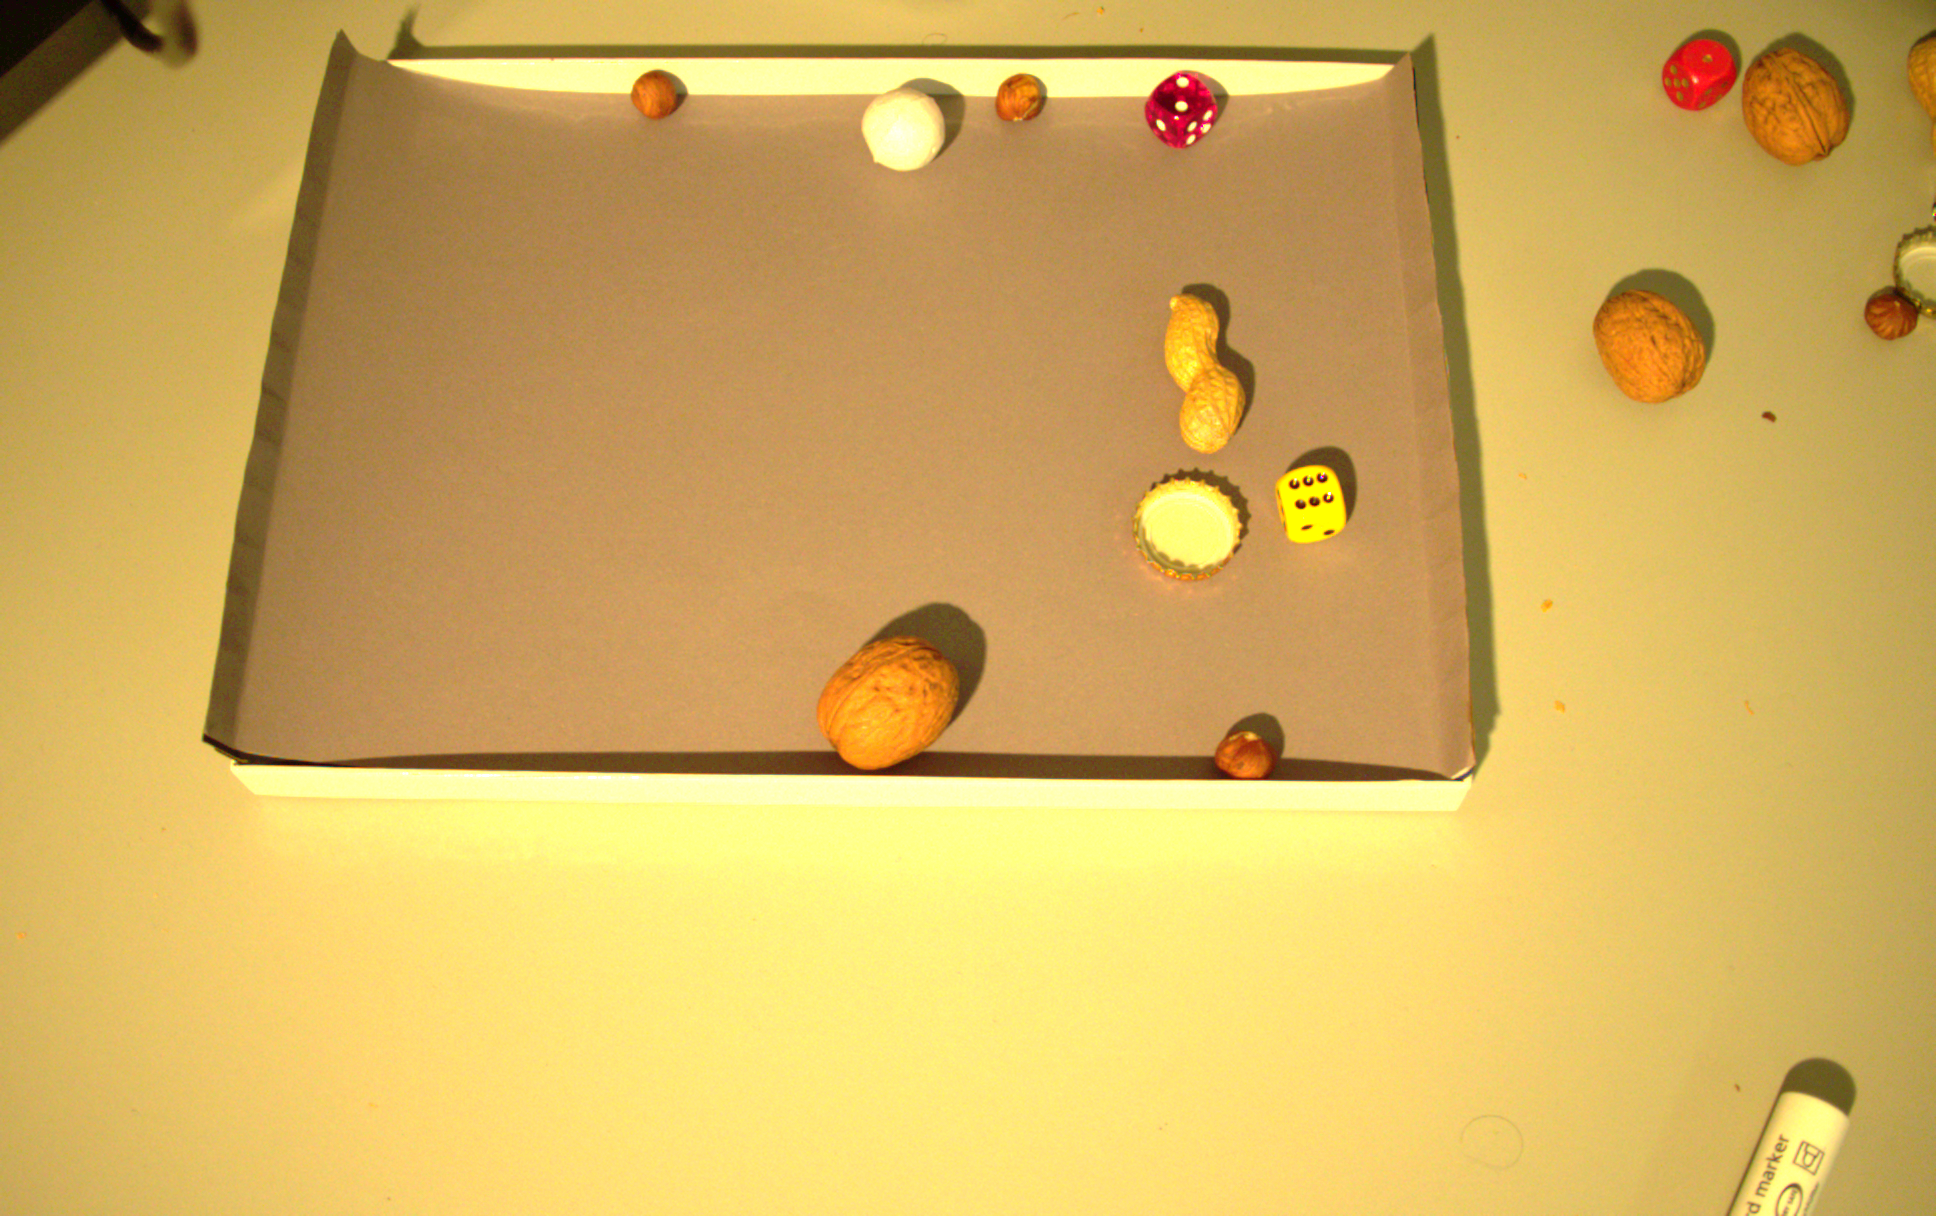
\includegraphics[width=\textwidth]{images/original_image_73}
   		\caption{Image to detect nuts inside the rectangle tray.}
   		\label{fig:original_image_73}
   	\end{subfigure}
   	\hfill
   	\begin{subfigure}[b]{0.475\textwidth}  
   		\centering 
   		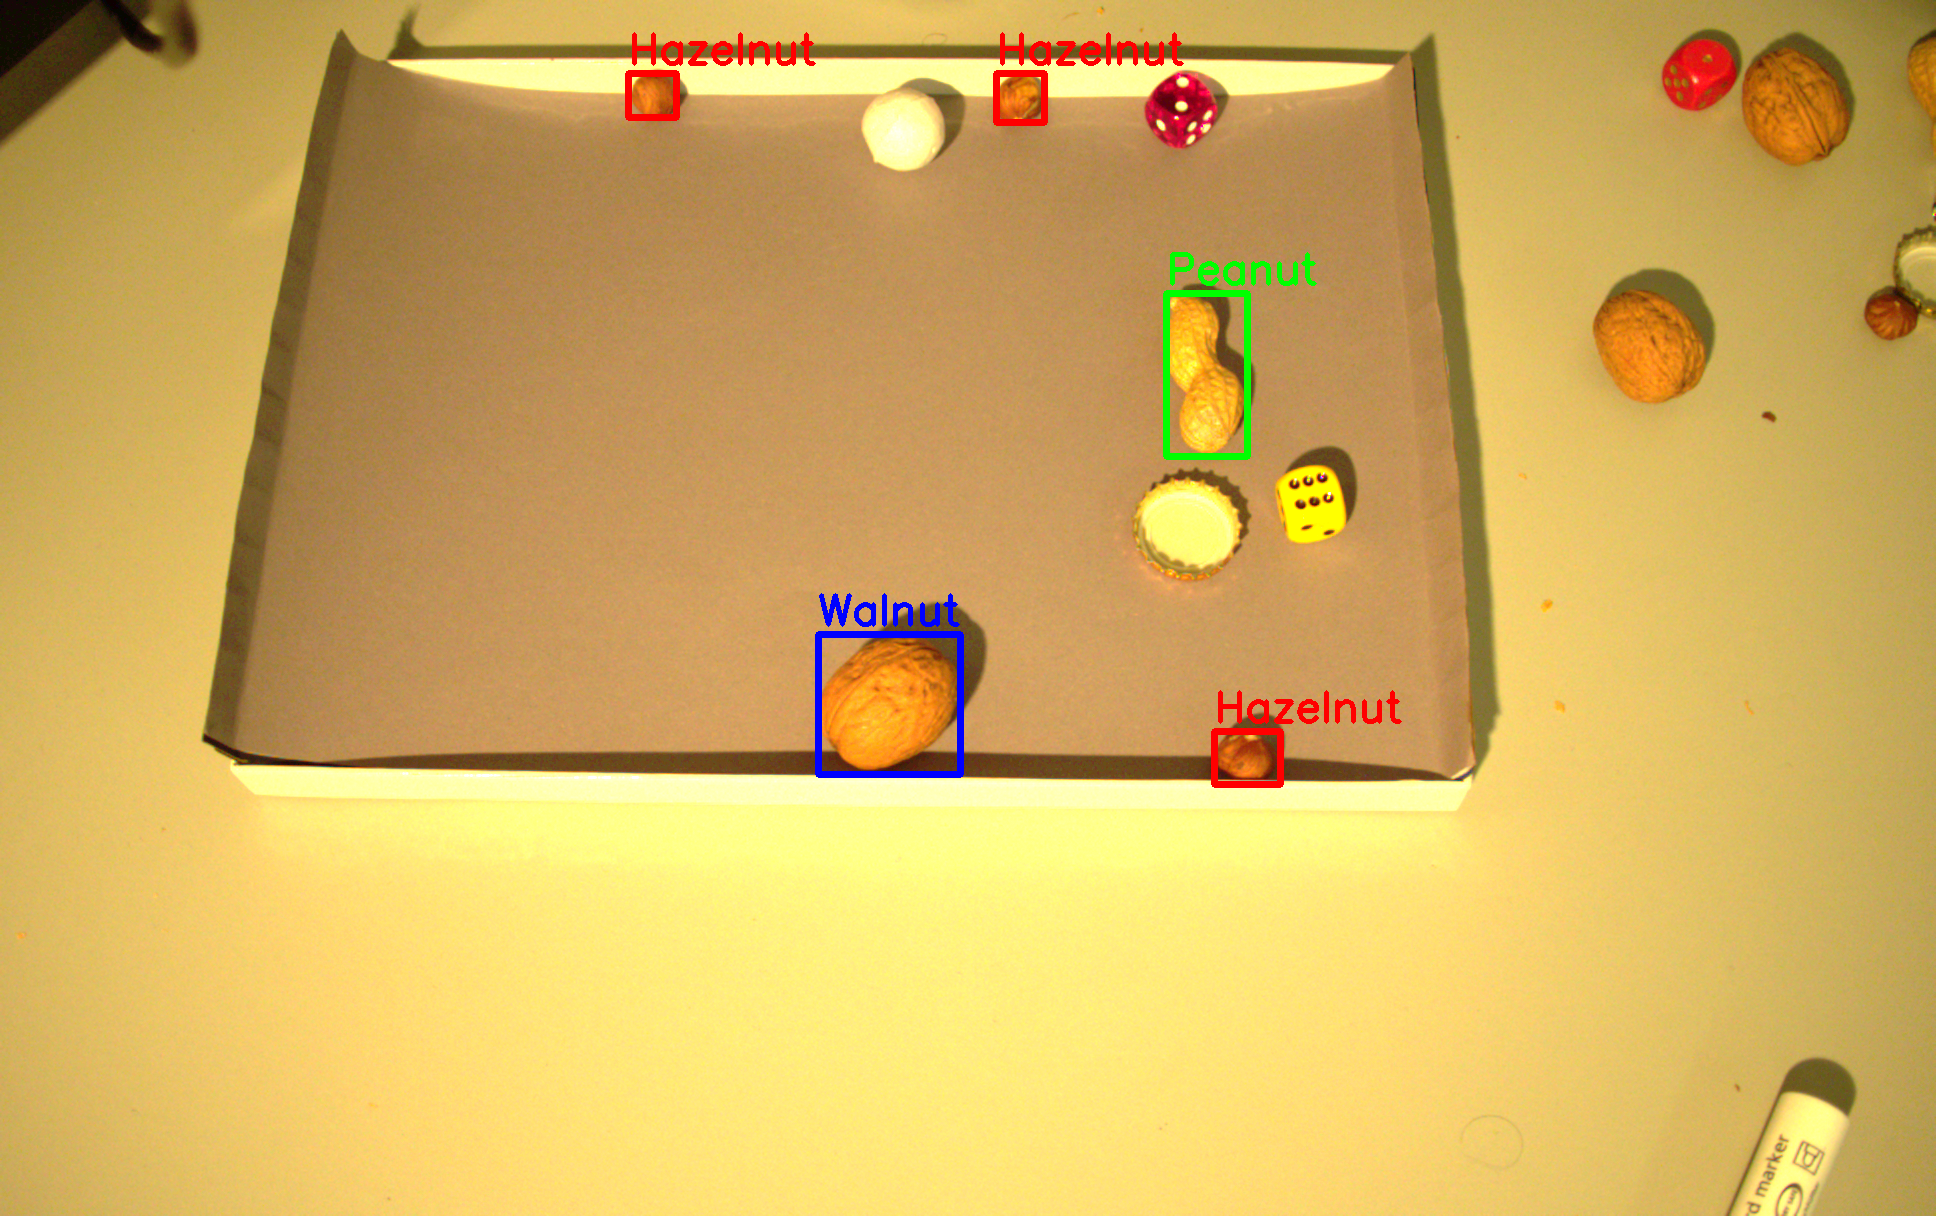
\includegraphics[width=\textwidth]{images/annotated_image_73_bb}
   		\caption{Image annotated with bounding box.}   
   		\label{fig:annotated_image_73_bb}
   	\end{subfigure}
   	\caption{Input image left side and the ground truth annotation on the right side to show the object of interest.}
   	\label{fig:ground_truth}
\end{figure*}

%This report aims to localize the nuts by their center of gravity instead of bounding box. 

%%%% MOTIVATION %%%
%Object detection used in many applications such as...


%%%% PROBLEM STATEMENT %%%%
Detecting objects of interest in the real-world such as peanut, walnut and hazelnut pose different challenging situations. Fundamental characteristic of the nuts is its shape, colour, texture and size. For example, nuts in our experiment shares similar hue but slightly different saturation and value. The texture features of the peanut and walnut can easily be confused by the classifier. Also, shape of peanut might look same but the width and height might vary. Desipte challenges from the object properties, camera and surrounding illumination plays an important role. The camera and the colour information from it impose several challenges. Figure \ref{fig:challenges} illustrates the different challenging situations such as low illumination, high illumination, shadow, occlusion and nuts outside the experimental tray in figure \ref{fig:original_image_73}.
\begin{figure*}
	\centering
	\begin{subfigure}[b]{0.3\textwidth}
		\centering
		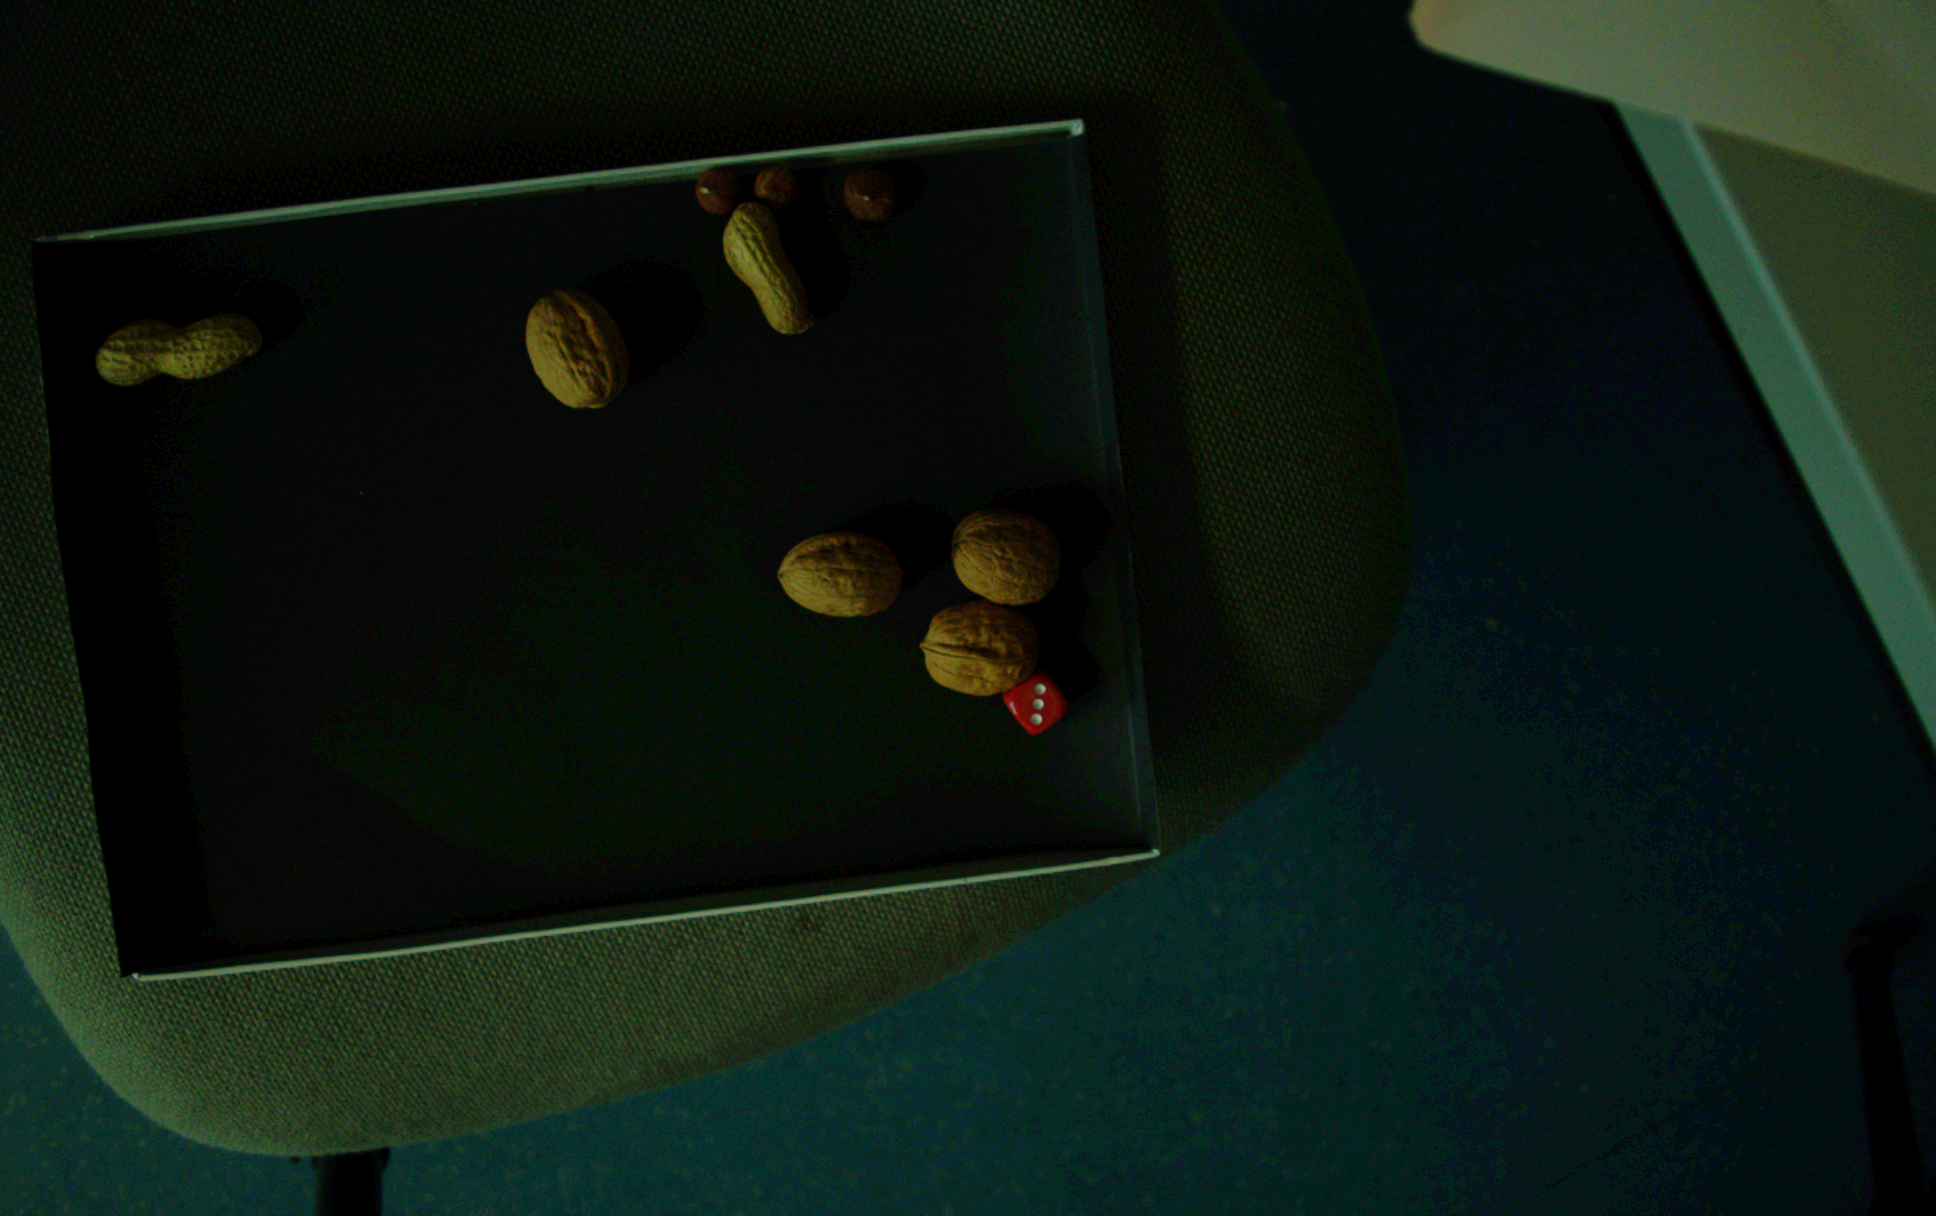
\includegraphics[width=\textwidth]{images/challenges/Low_illu_371.png}
		\caption{Poor illumination}
	\end{subfigure}
	\hfill
	\begin{subfigure}[b]{0.3\textwidth}  
		\centering 
		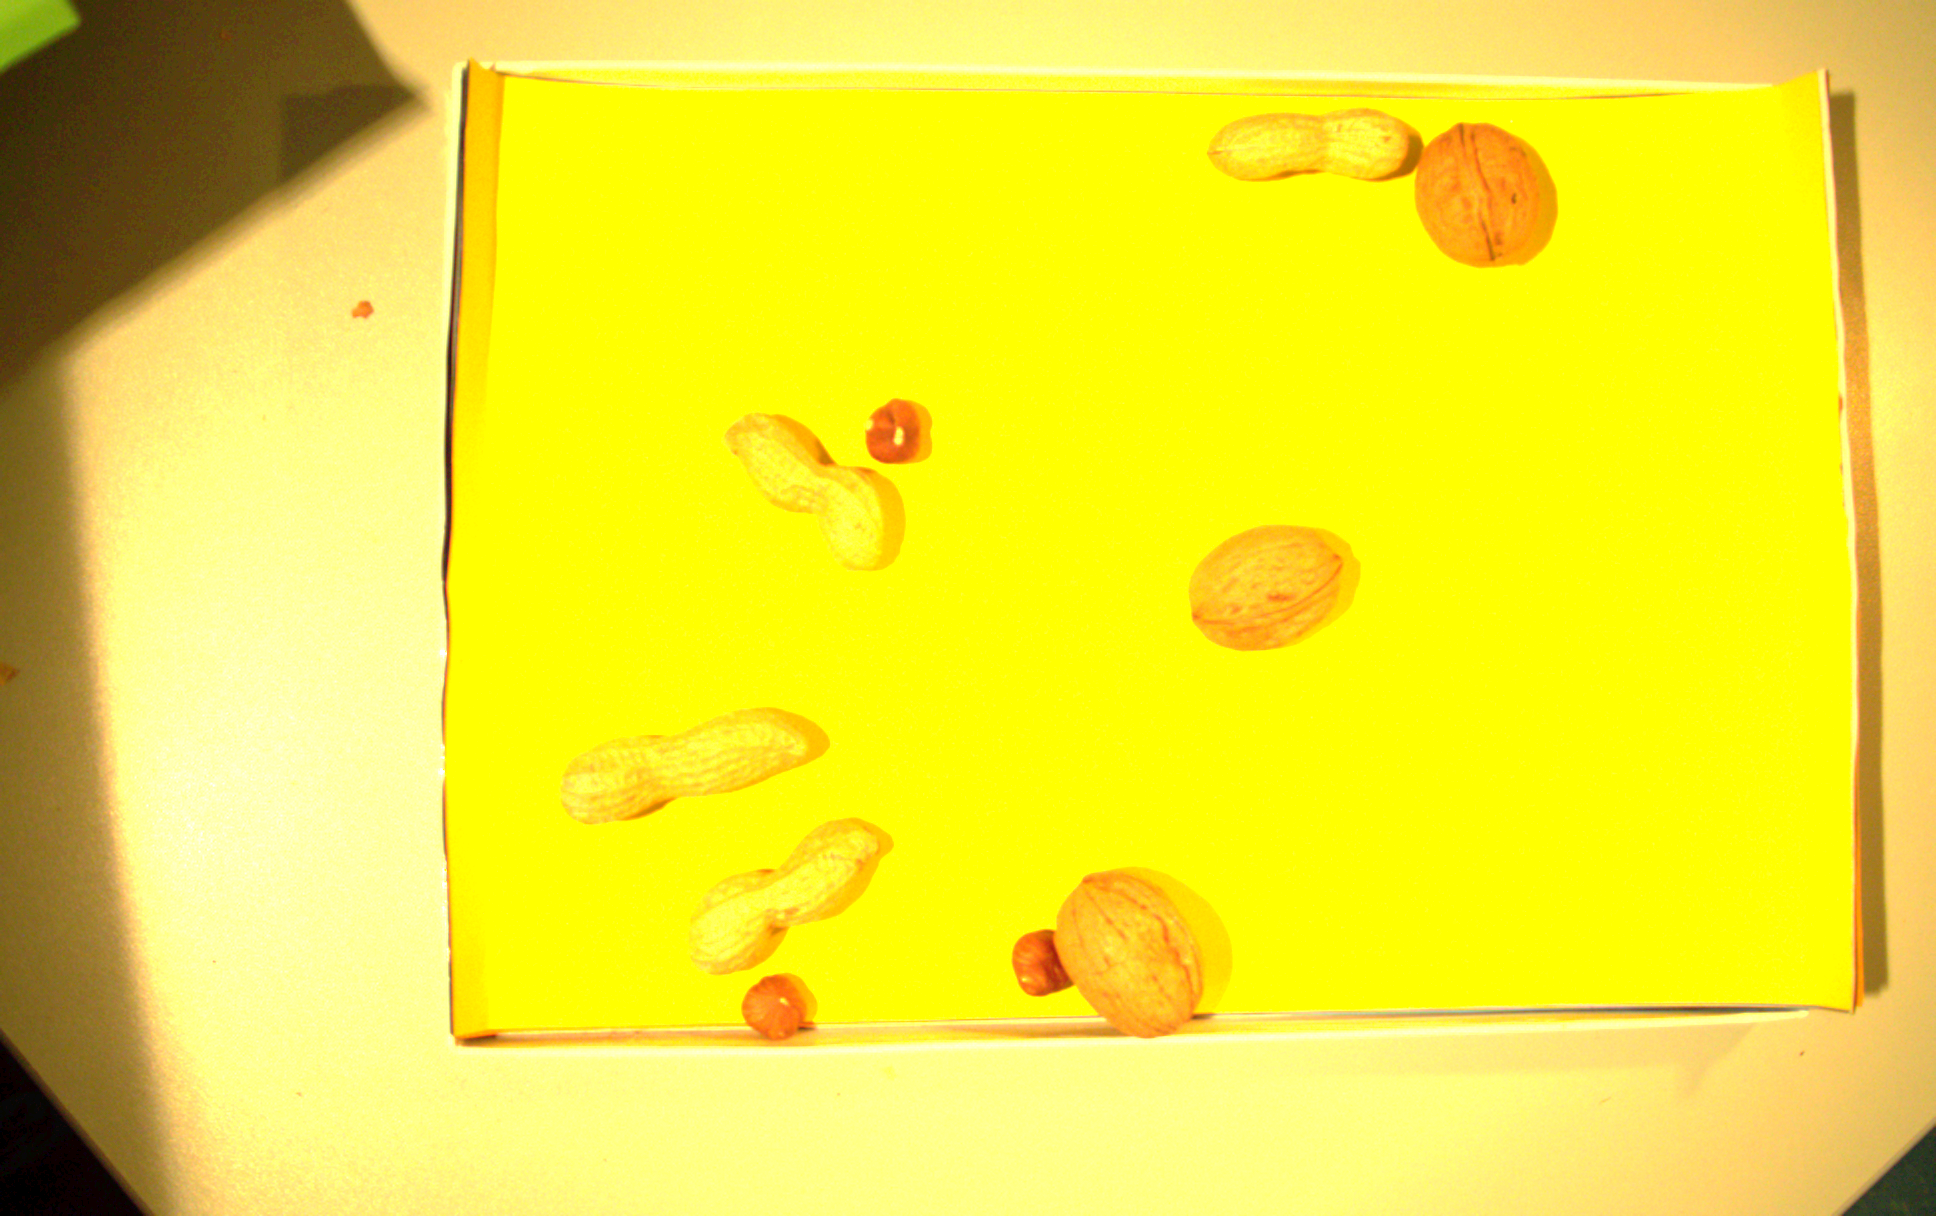
\includegraphics[width=\textwidth]{images/challenges/High_illu_336.png}
		\caption{High illumination} 
	\end{subfigure}
	\hfill
	\begin{subfigure}[b]{0.3\textwidth}  
		\centering 
		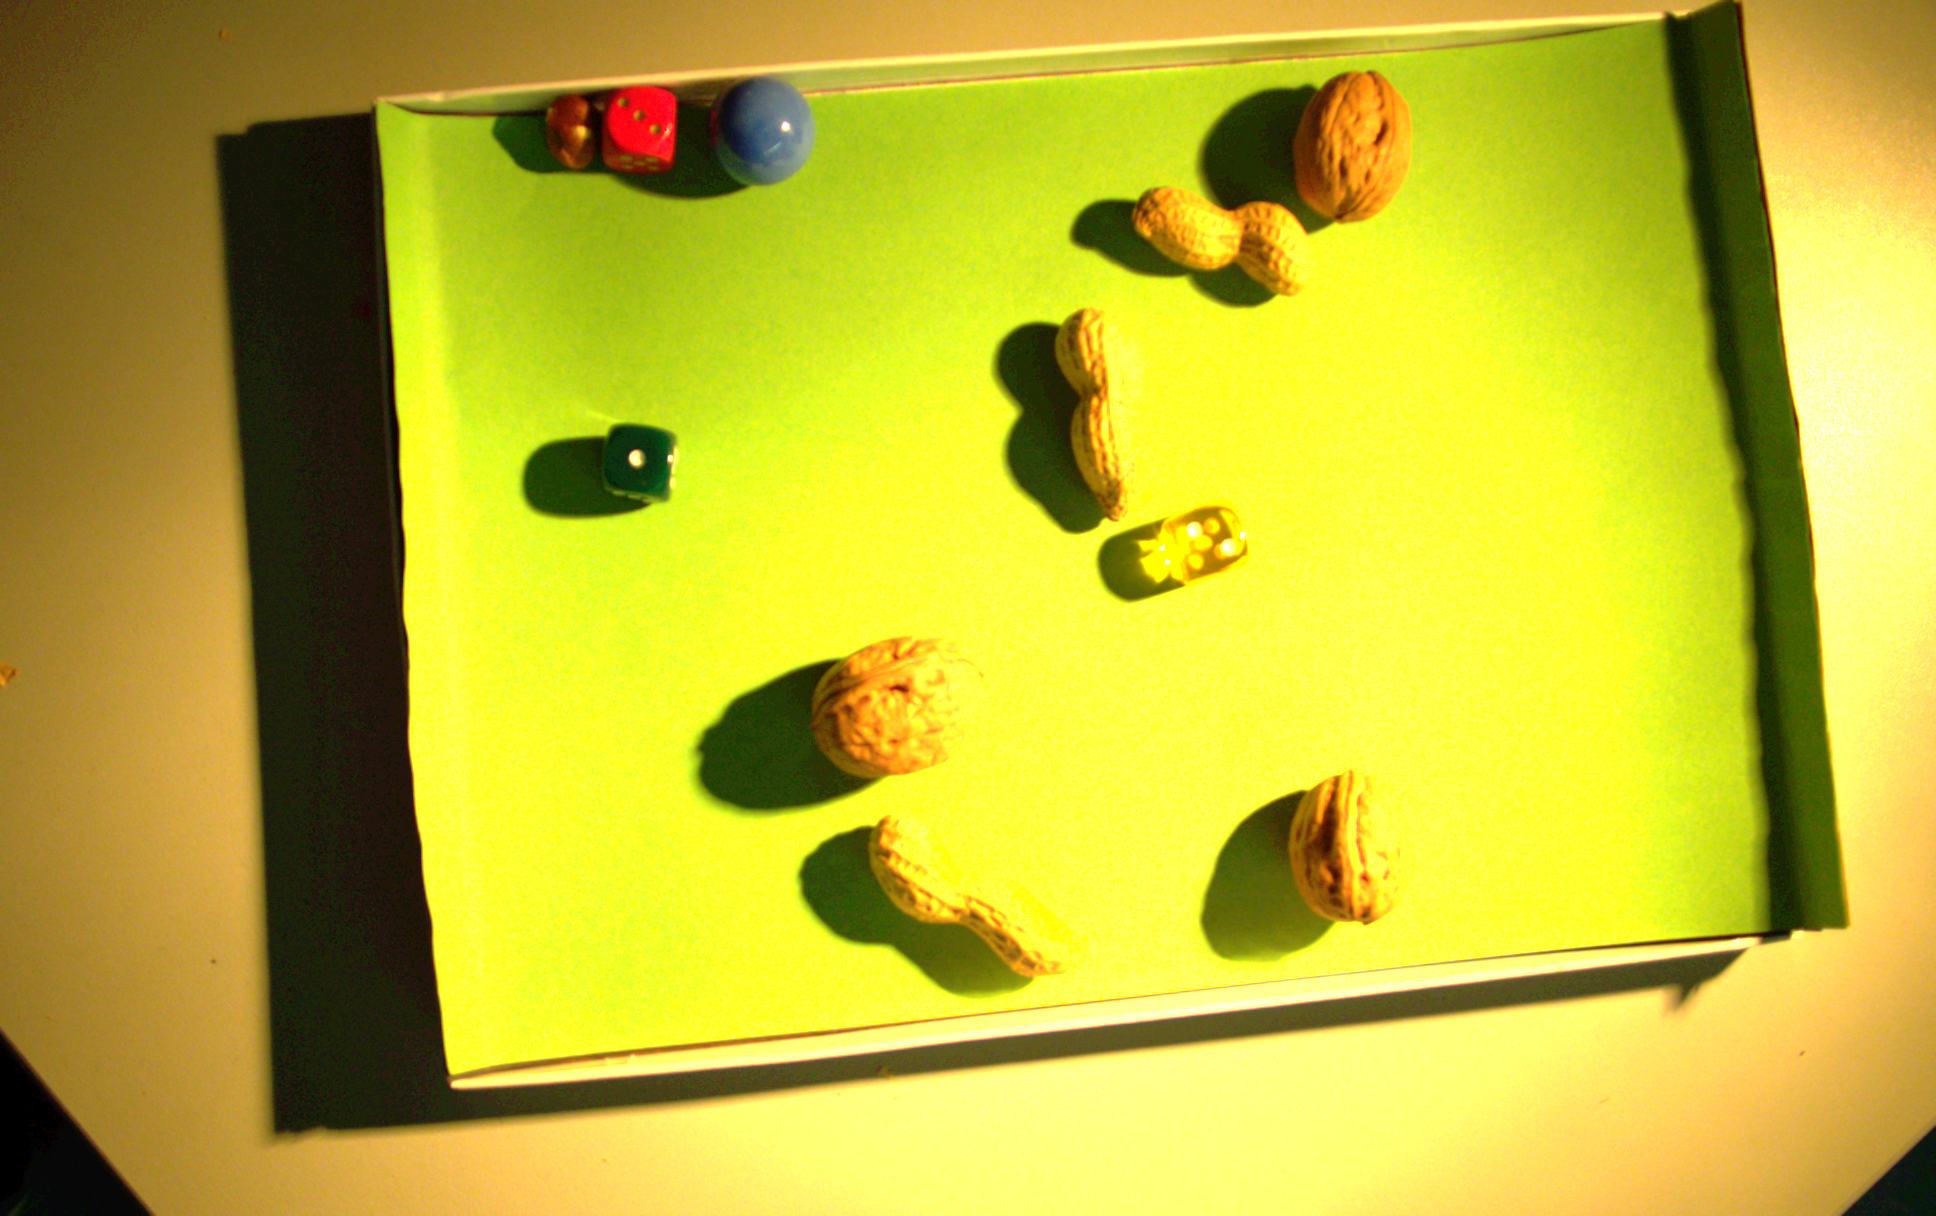
\includegraphics[width=\textwidth]{images/challenges/object_shadow_344.png}
		\caption{Object shadow} 
	\end{subfigure}
	\hfill
	\begin{subfigure}[b]{0.3\textwidth}  
		\centering 
		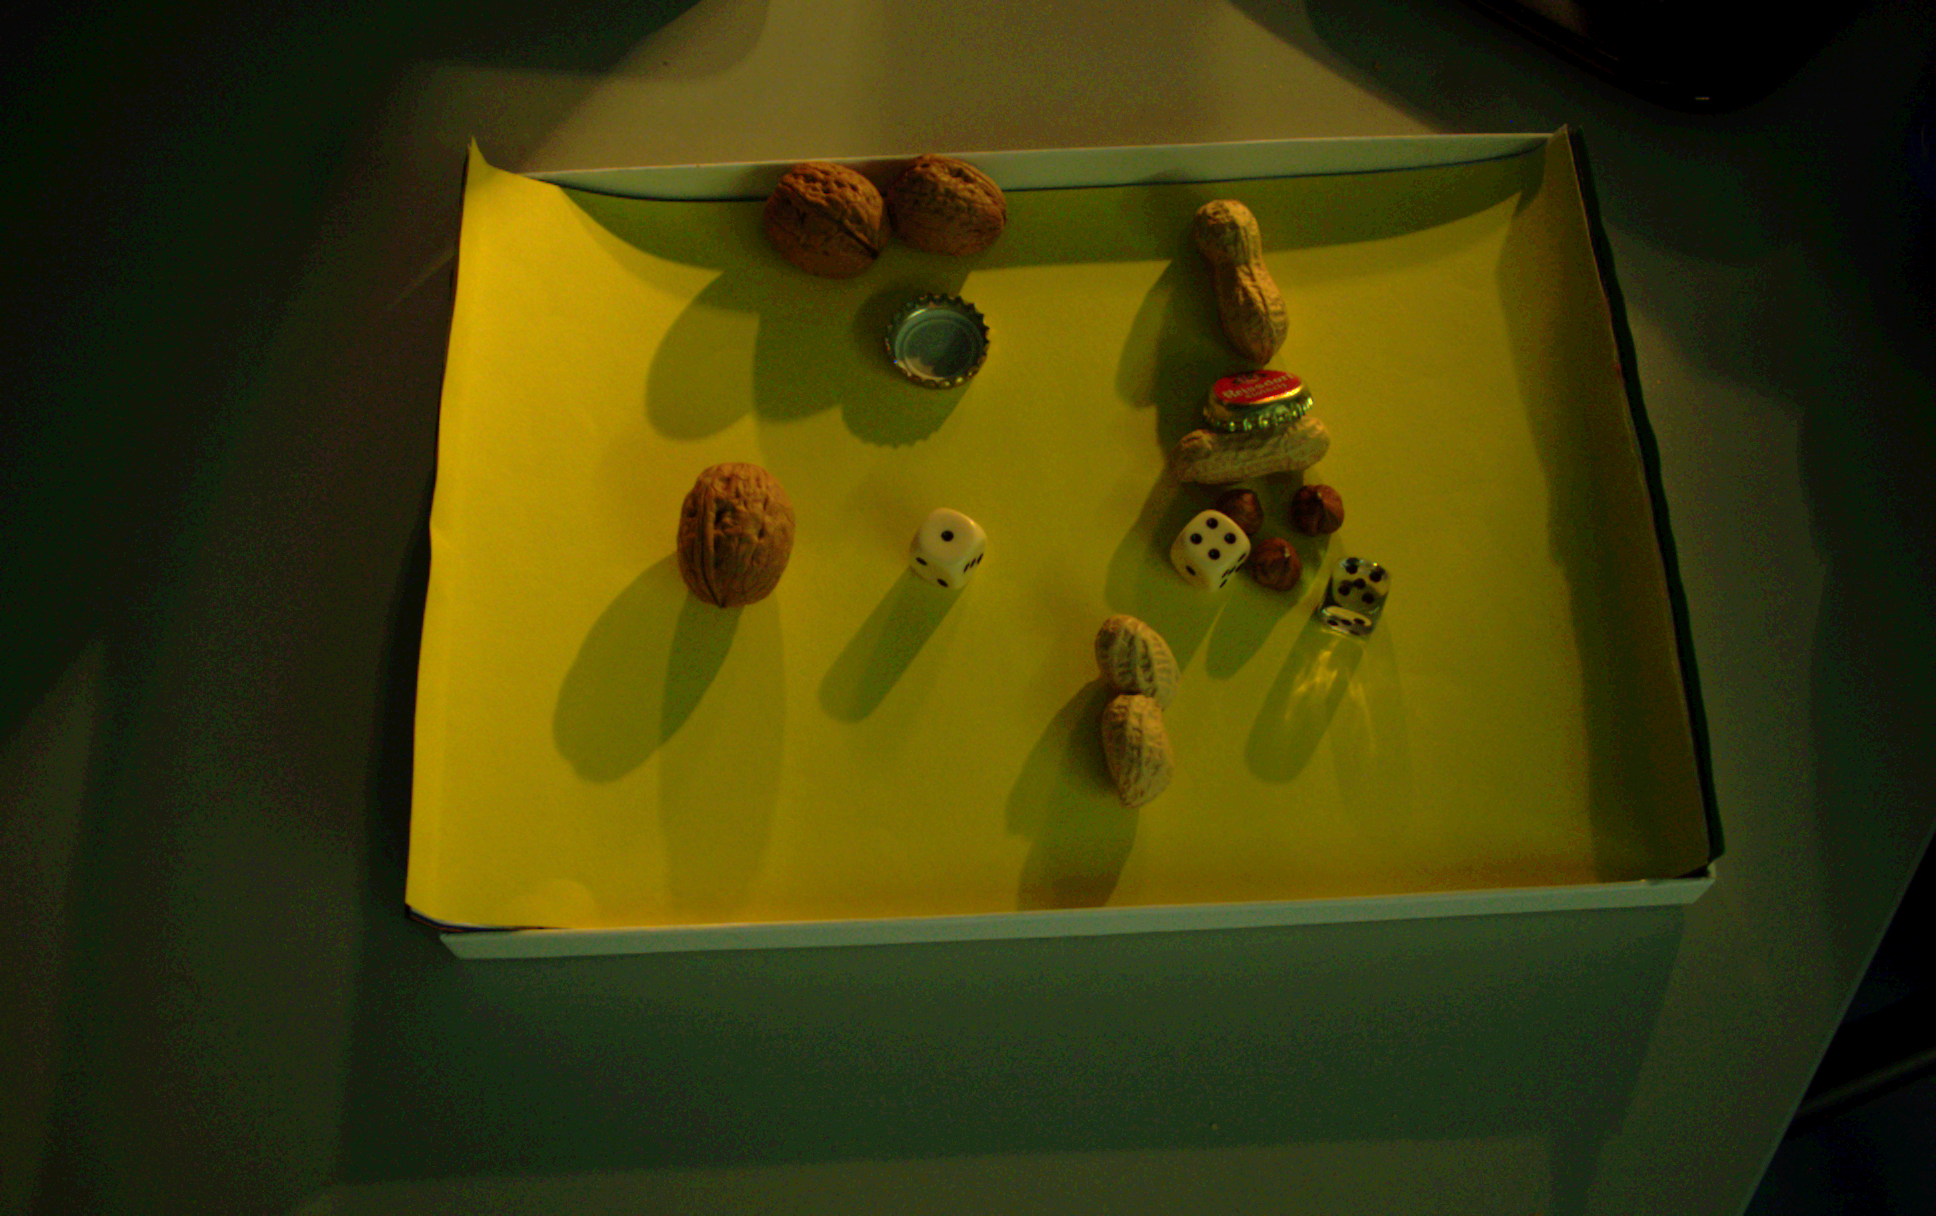
\includegraphics[width=\textwidth]{images/challenges/Cluttered_133.png}
		\caption{Cluttered objects} 
	\end{subfigure}
	\caption{Input image left side and the ground truth annotation on the right side to show the object of interest.}
	\label{fig:challenges}
\end{figure*}

Intro: Gentle start with basic terminology
Problem statement: Still unsolved because of number of challenges. Give images of occlusion, shadow, illumination, . Challenge is takes more time.
Motivation : Object detection is used in our daily life. Give many examples.
Proposed approach: Two stage: frame detection and object detection.
Explain Frame detection
Explain Object detection


Frame detection: 
\# Logic

1. find color histogram 
2. calculate difference of color histogram between previous and current frame. $(cv2.HISTCMP\_CORREL \& cv2.HISTCMP_KL\_DIV)$
3. we have two list of difference for entire video using two differnt methods
4. perform element wise subtraction of correlation with klDivergence -> new list
5. find value < 0. this is the frame with hands most of the time . add offset of 10 or 15 and you got it.
6. With too dark video you will never get. So suggetion is amplify klDiv by 10 and check if (value <0 and index < 15)

Write latex code or algorithm here

perfect situation - 267, 303, 316
low illumination - 282, 371, 12
High illumination - 336
shadow - 315

\section{Results}

\subsection{Speed of NN model}

\subsection{stable frame detection}

\subsection{Image processing}
rescalled, normalized, augmentation

\subsection{Training}

\subsection{Classification results}

\section{Conclusion}
Coclusion here

\section*{Acknowledgment}
WRITE YOUR ACK here

\bibliographystyle{unsrt} % Use the plainnat bibliography style
\bibliography{bibliography.bib} % Use the bibliography.bib file as the source of references
\end{document}
